\section{Certified finite-data phenomenon}
\label{sec:results}

\subsection{Four-transition common-map compatibility}

Let
\begin{equation}
D_4=\{\mathrm{TRAIN0},\mathrm{TRAIN1},H_1,H_2\}.
\end{equation}
A frozen whole-algebra physical CPTP map, denoted $\Phi_4$, was constructed for this dataset and then independently hostile-reviewed.  Its immutable artifact digest is
\begin{center}
\texttt{48abd5f52812ef7503cfdde92fe630b99ded9c10c4ef35d2c4edc8d934028125}.
\end{center}
The artifact contains all 49 central transfers and 5184 Kraus operators, with exact structural complete positivity and physical trace preservation after the frozen completion.  An independent exact certificate gives
\begin{equation}
\max_{j\in D_4}e_j(\Phi_4)
\le 0.006670414972746646\ldots <10^{-2}.
\label{eq:k4-upper}
\end{equation}
A reduction-free hostile ambient-dual certificate also gives the universal lower
\begin{equation}
\eps_*^{(4)}\ge 0.00028544924736174324\ldots .
\end{equation}
Hence the four-transition class is nonempty at the declared tolerance:
\begin{equation}
\Phi_4\in\F_4(10^{-2}).
\label{eq:phi4-feasible}
\end{equation}
This is a finite compatibility statement only.  At this stage $\Phi_4$ had no authority as an arbitrary-time law or as a prospectively validated predictor.

\subsection{Prospective failure of the frozen witness}

The exact artifact in \cref{eq:phi4-feasible} was frozen before the $F_1,F_2$ physical values were opened.  The outcome-blind schedule/provenance chain described in \cref{sec:physical} then selected the two pristine transitions.  On those transitions, simple rigorous lower certificates for the complete-source half-diamond error give
\begin{align}
e_{F_1}(\Phi_4)&\ge0.6246936110454476,\\
e_{F_2}(\Phi_4)&\ge0.6217658417777687.
\label{eq:phi4-forward-failure}
\end{align}
Both exceed the tolerance $10^{-2}$ by more than sixty-fold.  A fresh reviewer-owned full recomputation was subsequently executed and agreed with the banked result.  Therefore
\begin{equation}
\Phi_4\notin\F_6(10^{-2}).
\label{eq:phi4-not-f6}
\end{equation}
Crucially, \cref{eq:phi4-not-f6} says nothing by itself about whether $\F_6(10^{-2})$ is empty.

\begin{figure}[ht]
\centering
% Schematic custody/inference figure. Vertical layout prevents clipping and does not imply uniqueness.
\begin{tikzpicture}[
  node distance=0.55cm,
  >=Stealth,
  box/.style={draw,rounded corners,align=center,text width=0.80\linewidth,inner sep=5pt},
  arrow/.style={->,thick}
]
\node[box] (d4) {\textbf{Four exposed constraints}\\TRAIN0, TRAIN1, $H_1$, $H_2$};
\node[box,below=of d4] (p4) {$\exists\,\Phi_4\in\F_4(10^{-2})$\\selected physical CPTP witness};
\node[box,below=of p4] (freeze) {\textbf{Freeze $\Phi_4$ before unseen outcomes}\\then open prospectively selected $F_1,F_2$};
\node[box,below=of freeze] (fail) {\textbf{Prospective witness failure}\\
$e_{F_1}(\Phi_4)\ge 0.62469$, \quad
$e_{F_2}(\Phi_4)\ge 0.62177$};
\node[box,below=of fail] (d6) {\textbf{Only now enlarge the constraint set}\\TRAIN0, TRAIN1, $H_1$, $H_2$, $F_1$, $F_2$};
\node[box,below=of d6] (p6) {\textbf{Class remains compatible}\\
$\exists\,\Phi_6\in\F_6(10^{-2})$, \quad
$\max_j e_j(\Phi_6)\le0.00458264$};

\draw[arrow] (d4) -- node[right]{fit / certify} (p4);
\draw[arrow] (p4) -- (freeze);
\draw[arrow] (freeze) -- (fail);
\draw[arrow] (fail) -- node[right]{add opened tests as constraints} (d6);
\draw[arrow] (d6) -- node[right]{full unchanged class} (p6);
\end{tikzpicture}

\caption{The custody and inference sequence.  The four-transition data first certify one feasible witness $\Phi_4$, which is frozen before the unseen $F_1,F_2$ tests.  Failure of that fixed witness is then established prospectively.  Only after the new transitions are opened are they added to the constraint set, where a separate six-transition existence calculation certifies a witness $\Phi_6$.  The diagram does not imply that $\Phi_4$ was unique at K=4 or that $\Phi_6$ was obtained before $F_1,F_2$ were opened.}
\label{fig:fit-prediction}
\end{figure}

\subsection{Six-transition class compatibility after enlargement}

After $F_1$ and $F_2$ had been opened and their failure for $\Phi_4$ established, they were added as constraints rather than used to alter the physical model class.  The six-transition problem therefore uses exactly the same $\C$ as the K=4 problem.  An explicit whole-algebra map $\Phi_6$ was certified with artifact digest
\begin{center}
\texttt{c674e471c6bbad2e3376e53315d8e1e5cb83dbbb85f4120c7b5b8602b78f7e0a}.
\end{center}
Fresh hostile review independently reconstructed the complete-source residuals and certified the per-transition upper bounds in \cref{tab:k6-uppers}.

\begin{table}[ht]
\centering
\caption{Hostile-reviewed rigorous upper certificates for the accepted six-transition witness $\Phi_6$.}
\label{tab:k6-uppers}
\begin{tabular}{lr}
\toprule
transition & rigorous upper on $e_j(\Phi_6)$\\
\midrule
TRAIN0 & 0.0017360413721420206\\
TRAIN1 & 0.0017902995810885707\\
$H_1$ & 0.0017010819506354795\\
$H_2$ & 0.0022602480754981130\\
$F_1$ & 0.0045826386489339540\\
$F_2$ & 0.0044800043819739690\\
\bottomrule
\end{tabular}
\end{table}

The worst certified transition is $F_1$, so
\begin{equation}
\max_{j\in D_6}e_j(\Phi_6)
\le0.004582638648933954\ldots<10^{-2}.
\label{eq:k6-upper}
\end{equation}
A universal lower certificate, obtained from the subset TRAIN0+$F_1$+$F_2$ and lifted to the ambient whole-algebra problem, survived independent review at
\begin{equation}
\eps_*^{(6)}\ge0.002306082156934015\ldots .
\label{eq:k6-lower}
\end{equation}
Combining \cref{eq:k6-upper,eq:k6-lower} yields
\begin{equation}
\boxed{
0.002306082156934015\ldots
\le\eps_*^{(6)}
\le0.004582638648933954\ldots
<10^{-2}}
\label{eq:k6-bracket}
\end{equation}
and hence
\begin{equation}
\F_6(10^{-2})\neq\varnothing.
\label{eq:f6-nonempty}
\end{equation}

\begin{figure}[ht]
\centering
% Abstract set-membership schematic; boxes carry no metric/geometric meaning.
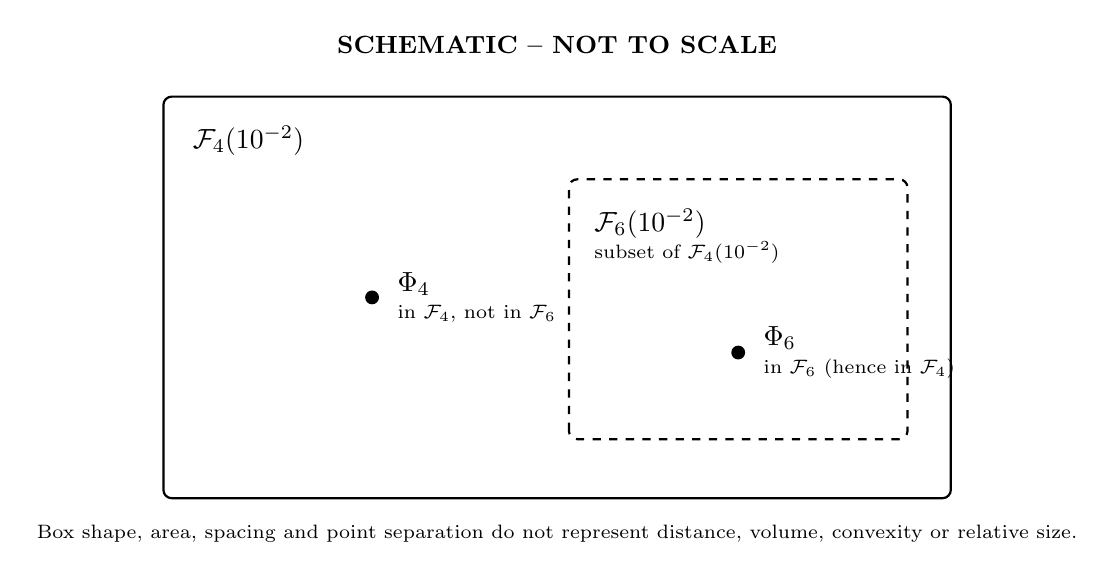
\begin{tikzpicture}[x=1cm,y=1cm]
  \node[font=\small\bfseries] at (0,3.35) {SCHEMATIC -- NOT TO SCALE};
  \draw[thick,rounded corners=3pt] (-5,-2.4) rectangle (5,2.7);
  \node[anchor=north west] at (-4.75,2.45) {$\mathcal F_4(10^{-2})$};

  \draw[thick,dashed,rounded corners=3pt] (0.15,-1.65) rectangle (4.45,1.65);
  \node[anchor=north west,align=left] at (0.35,1.40)
    {$\mathcal F_6(10^{-2})$\\[-2pt]\scriptsize subset of $\mathcal F_4(10^{-2})$};

  \fill (-2.35,0.15) circle (2.5pt);
  \node[anchor=west,align=left] at (-2.15,0.15)
    {$\Phi_4$\\[-2pt]\scriptsize in $\mathcal F_4$, not in $\mathcal F_6$};

  \fill (2.30,-0.55) circle (2.5pt);
  \node[anchor=west,align=left] at (2.50,-0.55)
    {$\Phi_6$\\[-2pt]\scriptsize in $\mathcal F_6$ (hence in $\mathcal F_4$)};

  \node[align=center,font=\scriptsize] at (0,-2.85)
    {Box shape, area, spacing and point separation do not represent distance, volume, convexity or relative size.};
\end{tikzpicture}

\caption{Schematic set-membership relation, not to scale.  Only $\F_6(10^{-2})\subseteq\F_4(10^{-2})$ and the marked membership/exclusion statements are asserted.  Box shape, area, spacing and point separation carry no geometric, metric, volume or convexity claim.}
\label{fig:nested-sets}
\end{figure}

\subsection{Central certified proposition}

\begin{proposition}[Frozen finite-system phenomenon]
\label{prop:central}
For the frozen $N=8$, $R2_{07}$ transition family and the full physical class $\C$ at tolerance $10^{-2}$:
\begin{enumerate}
\item $\Phi_4\in\F_4(10^{-2})$;
\item $\Phi_4\notin\F_6(10^{-2})$ because it fails both genuinely unseen $F_1,F_2$ transitions by the reviewed bounds in \cref{eq:phi4-forward-failure};
\item $\F_6(10^{-2})\neq\varnothing$, with the minimax bracket in \cref{eq:k6-bracket}.
\end{enumerate}
Therefore prospective failure of the frozen four-transition witness does not imply failure of six-transition common-map compatibility.
\end{proposition}

\begin{proof}
Item 1 follows from the certified bound \cref{eq:k4-upper}.  Item 2 follows because each lower bound in \cref{eq:phi4-forward-failure} is larger than $10^{-2}$.  Item 3 follows constructively from the certified whole-algebra witness $\Phi_6$ and \cref{eq:k6-upper}; the universal lower in \cref{eq:k6-lower} supplies the stated minimax bracket.  The final implication is immediate: one point $\Phi_4$ leaves the nested feasible set, while another point $\Phi_6$ remains.
\end{proof}

An additional deterministic consequence supplies the identification statement.  Since $D_4\subset D_6$, \cref{lem:nesting} gives $\F_6(10^{-2})\subseteq\F_4(10^{-2})$.  Therefore $\Phi_6\in\F_4(10^{-2})$ as well.  Together with $\Phi_4\in\F_4(10^{-2})$ and $\Phi_4\notin\F_6(10^{-2})$, this proves $\Phi_4\neq\Phi_6$ and shows that the K=4 tolerance-feasible set contains at least two distinct physical maps with sharply different certified prospective errors.  This is finite-data non-identification at the declared tolerance; it is not a theorem that every possible K=4 estimator has poor future risk.
